\documentclass{tufte-handout}
\usepackage{pgfplots}
\usepackage[dvipsnames]{xcolor}
\usepackage{ulem}
\usepackage{subcaption}
\usepackage{amssymb, amsmath, pgfplots, tabularx, siunitx}
\usepackage{algorithm}
\usepackage{booktabs}
\usepackage{makecell}
\usepackage{amsfonts}
\pgfplotsset{compat = newest}

\usepackage{tikz}
\usetikzlibrary{shadings}
\usetikzlibrary{positioning}
\usetikzlibrary{calc,arrows.meta}
\usetikzlibrary{shapes.misc}
\usepackage[most]{tcolorbox}
\usepgfplotslibrary{colormaps,patchplots}

\definecolor{wp-bg}{HTML}{FDF6EF}
\definecolor{wp-text}{HTML}{2D1B0E}
\definecolor{wp-primary}{HTML}{C24A3A}
\definecolor{wp-accent}{HTML}{D4952E}
\definecolor{wp-light}{HTML}{F0DECA}
\definecolor{wp-muted}{HTML}{C4A88A}
\definecolor{wp-dark}{HTML}{1A0F07}
\definecolor{wp-code}{HTML}{FDF2E4}

\pagecolor{wp-bg}
\color{wp-text}

\tikzset{basic/.style={draw,text width=1em,text badly centered}}
\tikzset{input/.style={basic,circle}}
\tikzset{weights/.style={basic,rectangle}}
\tikzset{functions/.style={basic,circle}}

\hypersetup{colorlinks=true,linkcolor=wp-primary,urlcolor=wp-accent}

\DeclareMathOperator*{\argmax}{argmax}
\DeclareMathOperator{\sg}{sg}

\title{World Models \\ A Survey of Internal Representations in Artificial Intelligence}
\author{Vitor N. Cabral de Oliveira \\ \href{mailto:vnco@cin.ufpe.br}{vnco@cin.ufpe.br}}
\date{\today}

\begin{document}

\maketitle
\begin{abstract}
    This document explores the concept of \textit{world models} --- internal representations
    that agents use to simulate and predict the environment. We cover the foundations, from
    cognitive science to modern deep learning implementations.
\end{abstract}

\newpage
\hypersetup{linkcolor=wp-text}
\tableofcontents
\hypersetup{linkcolor=wp-primary}
\newpage

\section{Introduction}

The ability to model the world is a cornerstone of intelligence. A \textbf{world model} is an
internal representation that an agent builds of its environment, enabling it to predict future
states, reason about consequences, and plan actions without direct trial and error in the real
world. This concept appears across cognitive science, robotics, control theory, and deep learning.

In artificial intelligence, world models have gained prominence through architectures that
explicitly separate perception, memory, and planning components. This document traces the
evolution of these ideas.

\section{Cognitive Foundations}

\paragraph{Mental Models in Psychology}
The notion of internal models traces back to Kenneth Craik's 1943 work \textit{The Nature of
Explanation}, where he proposed that organisms build ``small-scale models'' of reality to
anticipate events and test alternatives mentally.

\paragraph{Dorsal and Ventral Streams}
In neuroscience, the visual cortex is organized into two pathways:
\begin{itemize}
    \item \textbf{Ventral stream}: object recognition ("what")
    \item \textbf{Dorsal stream}: spatial processing ("where / how")
\end{itemize}

Modern world model architectures often mirror this separation between representational and
spatial reasoning pathways.

\section{Theoretical Frameworks}

\paragraph{Free Energy Principle}
Karl Friston's Free Energy Principle (FEP) posits that any self-organizing system restricted to a bounded number of 
states must minimize a mathematical quantity called \textit{variational free energy} to resist natural entropic decay and 
maintain its structural integrity~\nocite{friston2010}\sidenote{Friston, ``The free-energy principle: a unified brain theory?''}. 
Within this framework, world models emerge as a thermodynamic and statistical necessity. An agent maintains an internal generative 
model $p(o_t, s_t)$ over sensory observations $o_t$ and hidden environmental states $s_t$. By constructing a variational recognition 
density $q(s_t)$ that parameterizes its beliefs, the agent minimizes a tractable upper bound on sensory surprise (negative log-evidence):

\begin{equation}
    \begin{split}
        F &= \mathbb{E}_{q(s_t)}\left[\log q(s_t) - \log p(o_t, s_t)\right] \\
          &= D_{\mathrm{KL}}\left(q(s_t) \parallel p(s_t \mid o_t)\right) - \log p(o_t)
    \end{split}
    \label{eq:fep}
\end{equation}

Because the Kullback-Leibler ($D_{\mathrm{KL}}$) divergence is always non-negative, minimizing $F$ implicitly maximizes 
the evidence for the agent's internal model of the world, formalizing perception as variational inference.

\paragraph{Active Inference}
A direct corollary of the FEP is active inference, a paradigm asserting that action and perception are not 
distinct processes, but rather two sides of the same coin. While perception updates internal beliefs $q(s_t)$ to fit 
incoming data $o_t$, action alters the environment to force future data to conform to the model's prior expectations. 
Under active inference, an agent evaluates a policy $\pi$ by calculating its Expected Free Energy $G(\pi)$ across a future time horizon:

\begin{equation}
    G(\pi) = \sum_\tau \mathbb{E}_{q(o_\tau, s_\tau \mid \pi)}\left[\log q(s_\tau \mid \pi) - \log p(o_\tau, s_\tau)\right]
    \label{eq:active_base}
\end{equation}

By expanding this formulation, $G(\pi)$ can be cleanly decomposed into an epistemic value 
component (seeking out salient information to minimize ambiguity) and an instrumental value component (maximizing expected utility or 
preference satisfaction):

\begin{equation}
    G(\pi) \approx \sum_\tau \underbrace{-\mathbb{E}_{q(s_\tau \mid \pi)}\left[\mathcal{H}\left(q(o_\tau \mid s_\tau)\right)\right]}_{\text{Epistemic (Ambiguity Reduction)}} + \underbrace{\vphantom{\mathbb{E}_{q(s_\tau \mid \pi)}}D_{\mathrm{KL}}\left(q(o_\tau \mid \pi) \parallel p(o_\tau)\right)}_{\text{Instrumental (Risk Minimization)}}
    \label{eq:active_decomposition}
\end{equation}

This formulation structurally unifies the exploration-exploitation dilemma native to model-free reinforcement learning by 
grounding decision-making inside the agent's generative prediction loop.

\paragraph{Predictive Coding}
At the neurocomputational level, Rao and Ballard (1999) proposed that the mammalian cerebral cortex implements 
a hierarchical architecture optimizing this free-energy objective via a scheme known 
as \textit{predictive coding}~\nocite{rao1999}\sidenote{Rao and Ballard, ``Predictive coding in the visual cortex''}. 
In this structural hierarchy, higher cortical areas transmit top-down generative predictions to lower layers. The lower layers compare these predictions against raw sensory inputs or lower-level representations, generating a localized prediction error vector $\varepsilon_t = o_t - f(s_t)$. 

Crucially, rather than propagating raw, high-dimensional sensory 
states up the processing chain, the cortex exclusively transmits these residual error signals ($\varepsilon_t$) upward 
to adjust the latent states of higher-tier generative layers. This biological mechanism maps directly onto modern 
neural world models—such as Recurrent State-Space Models (RSSMs) and Predictive Coding Networks (PCNs)—where predictive 
reconstruction mismatches serve as the fundamental self-supervised learning signal for representation learning.

\begin{marginfigure}
\centering
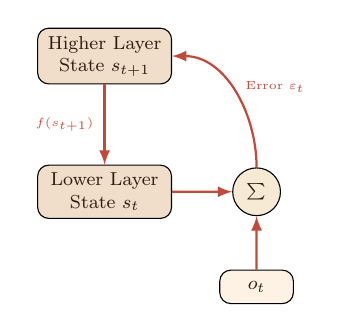
\begin{tikzpicture}[
    node distance=1.0cm and 0.8cm, % Condenses vertical and horizontal gaps
    auto, 
    font=\footnotesize,            % Drops base font size for small margin constraints
    >=latex,
    scale=0.85, transform shape    % Cleanly scales the entire canvas vector down 15%
  ]
  
  % Global Style Definitions (Slightly narrower widths for margins)
  \tikzset{
    layer/.style={draw, fill=wp-light, rounded corners, minimum width=2.0cm, minimum height=0.7cm, text=wp-text, align=center},
    error/.style={draw, circle, fill=wp-accent!20, minimum size=0.65cm, text=wp-text, font=\scriptsize},
    input/.style={draw, fill=wp-code, rounded corners, minimum width=1.1cm, minimum height=0.5cm, text=wp-text, align=center}
  }

  % Higher Level State
  \node (layer2) [layer] {Higher Layer \\ State $s_{t+1}$};
  
  % Lower Level State
  \node (layer1) [layer, below=of layer2, yshift=-0.2cm] {Lower Layer \\ State $s_t$};
  
  % Error Comparator node
  \node (comp) [error, right=of layer1, xshift=0.1cm] {$\sum$};

  % Sensory Observation input
  \node (obs) [input, below=of comp, yshift=0.2cm] {$o_t$};

  % Downward Generative Path (Predictions)
  \draw[->, wp-primary, thick] (layer2) -- node[left, font=\tiny, xshift=-1pt] {$f(s_{t+1})$} (layer1);
  \draw[->, wp-primary, thick] (layer1.east) -- (comp.west);
  
  % Raw Sensory Feed into the comparator
  \draw[->, wp-primary, thick] (obs.north) -- (comp.south);

  % Upward Error Propagation Path (Tighter control points for narrow margin)
  \draw[->, wp-primary, thick] (comp.north) .. controls +(up:0.8cm) and +(right:0.8cm) .. 
    node[right, midway, font=\tiny, xshift=1pt, yshift=2pt] {Error $\varepsilon_t$} (layer2.east);

\end{tikzpicture}
\caption{Hierarchical Predictive Coding loop scaled for the margin. Top-down predictions suppress lower-tier activity; calculated residuals ($\varepsilon_t$) ascend to update higher state representations.}
\label{fig:predictive_coding_margin}
\end{marginfigure}

\section{Two Paradigms: Predictive vs Generative World Models}

A useful distinction cuts across modern world model research: \textbf{predictive} world models
forecast specific future states given past context and actions, while \textbf{generative} world
models learn to sample novel trajectories or environments from a learned distribution, often
unconditionally or from minimal conditioning.

\subsection{Predictive World Models}

Predictive world models learn a transition dynamics function $f$ that maps current state and
action to a distribution over next states:

\begin{equation}
    p(s_{t+1} \mid s_t, a_t) = f_\theta(s_t, a_t)
    \label{eq:predictive}
\end{equation}

The purpose is \textit{forecasting}: given what has happened, what will happen next? These
models are trained to minimize prediction error and are typically used for planning and
model-based reinforcement learning --- the agent ``imagines'' the outcomes of candidate action
sequences before executing them.

Key representatives:
\begin{itemize}
    \item \textbf{Ha and Schmidhuber (2018)}: the original \textit{World Models} paper uses a
          VAE + RNN to predict future latent states. The model is trained on observation-action
          trajectories and used for planning in latent space.
    \item \textbf{LeCun's World Model (JEPA)}: Yann LeCun's proposed architecture for
          autonomous machine intelligence frames world models as a key component that predicts
          latent representations of future states, trained via self-supervised
          learning~\nocite{lecun2022}\sidenote{LeCun, ``A Path Towards Autonomous Machine Intelligence''}.
          The world model operates in representation space rather than pixel space, predicting
          abstract features of the environment.
    \item \textbf{Dreamer family (Hafner et al.)}: RSSM-based models that learn a latent dynamics
          model and train policies entirely on imagined trajectories.
\end{itemize}

\paragraph{JEPA: Joint Embedding Predictive Architecture}
LeCun's JEPA~\nocite{lecun2022}\sidenote{LeCun, ``Joint Embedding Predictive Architecture''} is a
self-supervised learning framework that forms the perceptual backbone of his proposed world
model. Unlike generative architectures that predict in pixel space (e.g., VAEs), JEPA predicts
in latent embedding space:

\begin{equation}
    \text{JEPA:} \quad \hat{s}_y = \text{Predictor}(s_x, \theta), \quad \mathcal{L} = \|\hat{s}_y - s_y\|^2
    \label{eq:jepa}
\end{equation}


where $s_x$ and $s_y$ are embeddings of two views (e.g., two crops of an image, or two
consecutive video frames) produced by a shared encoder, and the predictor estimates one from the
other. The key properties are:

\begin{itemize}
    \item \textbf{Representation collapse prevention}: a stop-gradient on the target encoder
          prevents the trivial constant solution, forcing the embeddings to be informative.
    \item \textbf{Abstraction}: by predicting in latent space, JEPA discards low-level,
          unpredictable details (pixel noise, texture variation) and captures high-level
          semantic structure.
    \item \textbf{Hierarchical extension}: stacked JEPA modules can operate at increasing
          levels of abstraction and timescales, mirroring the hierarchical predictive coding
          theory of cortex.
\end{itemize}

In the context of world models, JEPA provides the \textit{perception} component that maps raw
observations to a structured latent space where prediction becomes tractable. The world model
proper then operates on these latent representations, predicting future $s_y$ from past $s_x$
and actions.
Predictive world models are evaluated on prediction accuracy, planning success, and sample
efficiency in downstream tasks.

\begin{figure}[htbp]
\centering
\resizebox{\textwidth}{!}{%
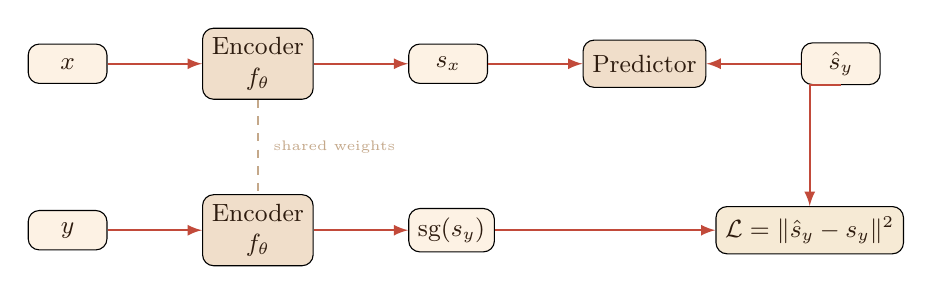
\begin{tikzpicture}[
    node distance=0.8cm and 1.2cm, 
    auto, 
    font=\small,
    >=latex   
  ]
  
  % Global Style Definitions
  \tikzset{
    box/.style={draw, fill=wp-light, rounded corners, minimum width=1.4cm, minimum height=0.6cm, text=wp-text, align=center},
    input/.style={draw, fill=wp-code, rounded corners, minimum width=1.0cm, minimum height=0.5cm, text=wp-text, align=center},
    loss/.style={draw, fill=wp-accent!20, rounded corners, minimum width=2.0cm, minimum height=0.6cm, text=wp-text, align=center}
  }

  % Top Path: Source Branch (x)
  \node (ix) [input] {$x$};
  \node (enc) [box, right=of ix] {Encoder \\ $f_\theta$};
  \node (sx) [input, right=of enc] {$s_x$};
  \node (pred) [box, right=of sx] {Predictor};
  \node (syhat) [input, right=of pred] {$\hat{s}_y$};

  % Bottom Path: Target Branch (y) - Positioned below the x path
  \node (iy) [input, below=of ix, yshift=-0.8cm] {$y$};
  \node (enc2) [box, right=of iy] {Encoder \\ $f_\theta$};
  \node (sg) [input, right=of enc2] {$\text{sg}(s_y)$};
  
  % Objective Node: Positioned inline with the bottom branch
  \node (loss) [loss, right=of sg, xshift=1.6cm] {$\mathcal{L} = \|\hat{s}_y - s_y\|^2$};

  % Connections for Top Path (x)
  \draw[->, wp-primary, thick] (ix) -- (enc);
  \draw[->, wp-primary, thick] (enc) -- (sx);
  \draw[->, wp-primary, thick] (sx) -- (pred);
  \draw[->, wp-primary, thick] (syhat) -- (pred);
  
  % Connections for Bottom Path (y)
  \draw[->, wp-primary, thick] (iy) -- (enc2);
  \draw[->, wp-primary, thick] (enc2) -- (sg);
  

  % Drops straight down from syhat.south, then turns horizontally into loss.north
  \draw[->, wp-primary, thick] (syhat.south) -| (loss.north);
  
  \draw[->, wp-primary, thick] (sg) -- (loss);

  % Shared Weight Indicator
  \draw[wp-muted, dashed, thick] (enc.south) -- (enc2.north) 
    node[midway, right, wp-muted, font=\tiny, xshift=2pt] {shared weights};

\end{tikzpicture}
}
\caption{LeCun's Joint Embedding Predictive Architecture. The context $x$ and target $y$ are mapped via a shared weight encoder[cite: 110]. The predictor operates entirely within the abstract latent space to compute $\hat{s}_y$ [cite: 110], which is compared against the stop-gradient ($\text{sg}$) representation of the target embedding to prevent representational collapse[cite: 111].}
\label{fig:jepa_horizontal}
\end{figure}

\subsection{Generative World Models}

Generative world models model the full joint distribution over environmental observation streams and actions. 
This formulation grants them the ability to \textit{sample} completely \textit{"novel"}, high-fidelity synthetic trajectories from scratch:

\begin{equation}
    p(o_1, \dots, o_T, a_1, \dots, a_T) = \prod_{t=1}^T p(o_t, a_t \mid o_{<t}, a_{<t})
    \label{eq:generative}
\end{equation}

Rather than committing to a localized, point-estimate calculation, generative world models capture the full 
multimodal distribution of possible environmental outcomes. They are typically optimized using unsupervised 
or self-supervised generative objectives—such as score-matching diffusion or autoregressive next-token 
prediction—making them highly capable simulators.

Key structural paradigms include:
\begin{itemize}
    \item \textbf{Google Genie}~\nocite{bruce2024}\sidenote{Bruce et al., ``Genie: Generative Interactive Environments''}: Trained on massive corpuses of unannotated video data, Genie uncovers an explicit 
          latent action space via an end-to-end video tokenizer coupled with a causal dynamics model. Given a 
          starting visual frame and an intended sequence of discrete latent actions, it synthesizes subsequent video 
          frames sequentially. At inference time, a single prompt image allows the framework to instantiate an 
          interactive, controllable 2D world on the fly.

    \item \textbf{High-Capacity Video Generation Models (GAIA-1, UniSim):} Large-scale transformers and temporal 
    diffusion networks learn foundational physical properties by directly predicting high-dimensional frame dynamics. 
    Though historically treated purely as media synthesis systems, these architectures implicitly learn rich intuitive 
    physics, object permanence, and temporal causality directly from raw pixel data.

\end{itemize}

Generative world models are primarily evaluated on sample quality, distributional diversity, 
long-horizon temporal consistency, and their capacity for out-of-distribution compositional generalization.

\begin{table}[htbp]
\centering
\small
% Explicitly setting smaller, static widths for the columns prevents margin spill
\begin{tabular}{l p{3.2cm} p{3.2cm}}
\toprule
\textbf{Dimension} & \textbf{Predictive Paradigm} & \textbf{Generative Paradigm} \\
\midrule
\textbf{Primary Objective} & Minimize latent feature distance & Maximize joint log-likelihood \\
\textbf{Output Type} & Abstract state target prediction & Full observation stream sampling \\
\textbf{Learning Signal} & Feature alignment or energy scores & Pixel reconstruction / token loss \\
\textbf{Downstream Utility} & Local look-ahead planning \& MBRL & Ambient environment simulation \\
\textbf{Core Vulnerability} & Susceptible to representation collapse & High computational sample cost \\
\bottomrule
\end{tabular}
\caption{Key differences between predictive and generative world models.}
\label{tab:paradigms}
\end{table}

\subsection{Bridging the Two Views}

The boundary dividing these two modeling paradigms is fundamentally fluid. Modern deep architectures frequently hybridize both frameworks to exploit their complementary strengths. 
For instance, DeepMind's \textit{Dreamer} utilizes an underlying generative model over compact latent configurations, but applies it predictively to generate localized 
rollouts for policy optimization. Conversely, Google's \textit{Genie} integrates a predictive, action-conditioned latent controller inside a wider autoregressive generative pipeline.

Importantly, Yann LeCun's JEPA explicitly rejects generative construction loops in favor of a purely predictive, energy-based abstract scoring predictor to prevent representational
hallucinations. However, as Jürgen Schmidhuber historically demonstrated, the fundamental mechanics remain deeply entangled: any world model tracking transitions can generate 
experiences iteratively by feeding its previous outputs back into its input layers, and any high-capacity generative sampler implicitly encapsulates an accurate predictive 
model of the underlying physical landscape. The taxonomy is therefore defined by the choice of learning signal and representational abstraction level 
rather than a rigid architectural barrier.

\subsection{Schmidhuber's Theoretical Foundations}

Jürgen Schmidhuber's contributions to world models span decades, predating the deep learning
era. His work provides the theoretical bedrock for both predictive and generative paradigms.

\paragraph{Artificial Curiosity (1991)}
Schmidhuber formalized \textit{artificial curiosity}~\nocite{schmidhuber1991}\sidenote{Schmidhuber, ``A Possibility for Implementing Curiosity and Boredom in Model-Building Neural Controllers''} as an
intrinsic reward signal that drives an agent to seek experiences that improve its world model.
The agent is rewarded for prediction errors --- but only those that are \textit{learnable},
avoiding both predictable noise and inherently unpredictable chaos. This creates a lifelong
learning loop where the world model and the exploration policy co-develop:

\begin{equation}
    \text{curiosity reward} = \|\hat{s}_{t+1} - s_{t+1}\|^2 \quad \text{(only if learnable)}
    \label{eq:curiosity}
\end{equation}

This principle directly inspired modern exploration bonuses in model-based RL (e.g., Intrinsic
Curiosity Module by Pathak et al., 2017).

\paragraph{Computational Principles of Creativity (2012)}
Schmidhuber extended the same framework to explain creativity and humor~\nocite{schmidhuber2012}\sidenote{Schmidhuber, ``Formal Theory of Creativity, Fun, and Intrinsic Motivation''}. A creator (artist,
scientist, comedian) generates works that induce a learnable compression progress in the
observer's world model. The ``fun'' or ``beauty'' of an experience is proportional to the
learning progress it produces --- the improvement in the observer's ability to predict or
compress the data.

\paragraph{Predictive World Models as Universal}
Schmidhuber argues that any powerful AI will necessarily build predictive world models because
they are required for:
\begin{itemize}
    \item \textbf{Planning}: simulating action outcomes before committing to one.
    \item \textbf{Explanation}: compressing sensory data into causal structures.
    \item \textbf{Transfer}: abstracting invariant patterns across different tasks.
\end{itemize}

The 2018 \textit{World Models} paper by Ha and Schmidhuber was a direct implementation of these
decades-old principles, showing that a VAE + RNN + controller trained with a simple evolutionary
strategy could solve RL tasks by ``dreaming'' --- planning in latent space.

\section{Foundational Architectures}

The modern formulation of world models in deep learning was popularized by Ha and Schmidhuber
(2018) in their paper \textit{World Models}~\nocite{ha2018}\sidenote{Ha and Schmidhuber, ``World Models''}. Their architecture consists of three components:


\begin{enumerate}
    \item \textbf{Vision (V)}: A variational autoencoder (VAE) that compresses high-dimensional
          observations into a compact latent representation.
    \item \textbf{Memory (R)}: A recurrent neural network (typically an LSTM or GRU) that
          predicts future latent states given actions, enabling temporal reasoning.
    \item \textbf{Controller (C)}: A policy network that selects actions based on the latent
          trajectory, often trained with a simple linear model or evolutionary strategies.
\end{enumerate}

\begin{marginfigure}[-3.0cm]
\centering
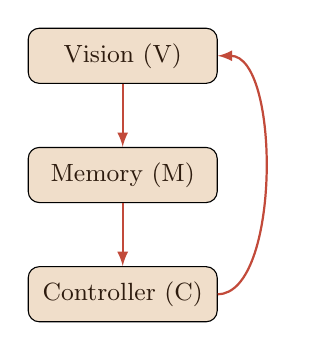
\begin{tikzpicture}[
    node distance=0.8cm, % Compact vertical gaps matching your other margin figures
    auto, 
    font=\small,
    >=latex
  ]
  
  % Global Style Definitions matching previous architectural motifs
  \tikzset{
    comp/.style={draw, fill=wp-light, rounded corners, minimum width=2.4cm, minimum height=0.7cm, text=wp-text, align=center}
  }

  % Vertical Node Registry
  \node (v) [comp] {Vision (V)};
  \node (m) [comp, below=of v] {Memory (M)};
  \node (c) [comp, below=of m] {Controller (C)};

  % Downward feed-forward pipeline (Using your designated wp-primary)
  \draw[->, wp-primary, thick] (v) -- (m);
  \draw[->, wp-primary, thick] (m) -- (c);
  
  % Upward feedback control loop
  \draw[->, wp-primary, thick] (c.east) .. controls +(right:0.8cm) and +(right:0.8cm) .. (v.east);

\end{tikzpicture}
\caption{Ha and Schmidhuber's three-component architecture.}
\label{fig:wm-arch}
\end{marginfigure}

\paragraph{Latent State Representation}
The VAE maps the observation $x_t$ to a latent Gaussian distribution $z_t \sim
\mathcal{N}(\mu_t, \sigma_t)$. The memory model predicts the next latent state given the
current state and action:

\begin{equation}
    \hat{z}_{t+1} = f_\theta(z_t, a_t)
    \label{eq:pred}
\end{equation}

The controller then selects actions $a_t = \pi(z_t)$ to maximize cumulative reward, often
trained separately using the latent space rather than raw pixels.

\subsection{Planning in Latent Space}

A key advantage of world models is the ability to plan by \textit{imagining} future trajectories
in latent space, avoiding expensive pixel-level simulation. This is formalized as:

\begin{algorithm}[h]
    \caption{Latent Planning with World Model}
        \textbf{Given}: Vision model $V$, Memory model $R$, current latent $z_t$ \\
        \textbf{For} each candidate action sequence $(a_t, ..., a_{t+H})$: \\
        \quad $z \leftarrow z_t$ \\
        \quad \textbf{For} $k = 1$ to $H$: \\
        \quad\quad $z \leftarrow f_\theta(z, a_{t+k-1})$ \\
        \quad\quad Accumulate reward $r_k$ \\
        \quad Select sequence with highest total reward \\
        \quad Execute first action $a_t$
\end{algorithm}

\subsection{Dreamer}

Building on Ha and Schmidhuber, Dreamer (Hafner et al., 2020) extends world models by
integrating the learning of all three components end-to-end using gradients through
dynamics~\nocite{hafner2020}\sidenote{Hafner et al., ``Dream to Control: Learning Behaviors by Latent Imagination''}.

The Dreamer architecture uses:
\begin{itemize}
    \item A \textbf{RSSM} (Recurrent State-Space Model) that combines deterministic and
          stochastic recurrent states.
    \item \textbf{Latent imagination}: value and policy networks trained entirely on imagined
          trajectories.
    \item \textbf{Behavior learning} via actor-critic in the compact latent space.
\end{itemize}

\subsection{Contrastive Approaches}

More recent work explores contrastive objectives for learning world models without generative
decoding. Approaches like CURL~\nocite{laskin2020}\sidenote{Laskin et al., ``CURL: Contrastive Unsupervised Representations for Reinforcement Learning''} use instance discrimination to shape the
latent space, avoiding the computational cost of reconstructing high-dimensional observations.

\section{Technical Deep Dive}

\subsection{Recurrent State-Space Model (RSSM)}

The RSSM, introduced by Hafner et al. in Dreamer, combines deterministic and stochastic
recurrent paths. At each time step $t$, the model computes:

\begin{align}
    h_t &= f_\phi(h_{t-1}, z_{t-1}, a_{t-1}) \quad \text{(deterministic)} \\
    z_t &\sim \mathcal{N}(\mu_\phi(h_t), \sigma_\phi(h_t)) \quad \text{(stochastic)} \\
    \hat{o}_t &= g_\phi(h_t, z_t) \quad \text{(observation reconstruction)}
\end{align}

The key insight is the hybrid state: the deterministic path $h_t$ carries long-range temporal
dependencies, while the stochastic path $z_t$ captures multimodal future outcomes. This avoids
the posterior collapse common in purely stochastic recurrent models.

\subsection{DreamerV2 and V3}

\paragraph{DreamerV2}
DreamerV2~\nocite{hafner2021}\sidenote{Hafner et al., ``Mastering Atari with Discrete World Models''} introduced several critical innovations:
\begin{itemize}
    \item \textbf{Discrete latents}: replacing Gaussian $z_t$ with categorical distributions
          enabled richer multimodal representations.
    \item \textbf{KL balancing}: separate KL coefficients for the prior and posterior to
          prevent the posterior from collapsing to the prior.
    \item \textbf{Two-hot reward prediction}: predicting reward distributions rather than
          point estimates improved value learning.
\end{itemize}

The discrete latent representation $z_t \in \{1, ..., K\}^D$ uses straight-through gradients,
allowing backpropagation through the categorical sampling step:

\begin{equation}
    z_t = \text{one-hot}\left(\argmax_k \pi_k\right) + \pi - \text{sg}(\pi)
\end{equation}

where $\pi$ are the logits and $\text{sg}$ denotes stop-gradient.

\paragraph{DreamerV3}
DreamerV3~\nocite{hafner2023}\sidenote{Hafner et al., ``DreamerV3: Mastering Diverse Domains through World Models''} further generalized the approach to work across hundreds of environments with a
single set of hyperparameters --- a major milestone in robust world model learning. Key
additions include:

\begin{itemize}
    \item \textbf{Symlog predictions}: using the symlog transformation
          $\text{symlog}(x) = \text{sign}(x)\log(|x|+1)$ to handle targets of varying scale
          without normalization.
    \item \textbf{Free bits}: a KL regularizer that allows the posterior to stay close to the
          prior without collapsing, enforced by a minimum KL divergence.
    \item \textbf{Normalized predictions}: reward and value heads predict distributions
          normalized by running statistics, enabling cross-domain transfer.
\end{itemize}

\section{Transformer-Based World Models}

The success of transformers in sequence modeling has inspired a new generation of world model
architectures that replace recurrent dynamics with attention mechanisms.

\subsection{IRIS}
IRIS~\nocite{micheli2023}\sidenote{Micheli et al., ``Transformers are Sample Efficient World Models''} replaces the recurrent memory with a GPT-style transformer operating on discrete visual tokens:

\begin{figure*}[htbp] % Note the asterisk (*)
\centering
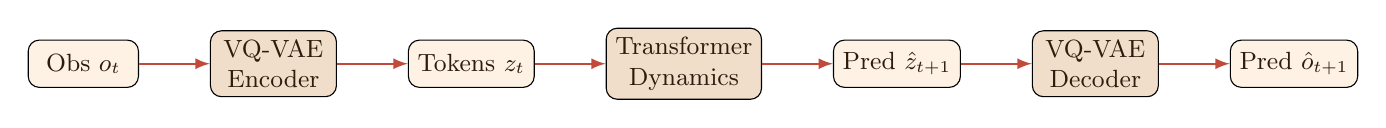
\begin{tikzpicture}[
    node distance=0.6cm and 0.9cm, % Slightly tightened for a perfect fit
    auto, 
    font=\small,
    >=latex
  ]
  
  \tikzset{
    block/.style={draw, fill=wp-light, rounded corners, minimum width=1.6cm, minimum height=0.7cm, text=wp-text, align=center},
    embed/.style={draw, fill=wp-code, rounded corners, minimum width=1.4cm, minimum height=0.6cm, text=wp-text, align=center}
  }

  % Nodes arranged horizontally left-to-right
  \node (obs)   [embed] {Obs $o_t$};
  \node (vq)    [block, right=of obs] {VQ-VAE \\ Encoder};
  \node (tok)   [embed, right=of vq] {Tokens $z_t$};
  \node (trans) [block, right=of tok] {Transformer \\ Dynamics};
  \node (pred)  [embed, right=of trans] {Pred $\hat{z}_{t+1}$};
  \node (dec)   [block, right=of pred] {VQ-VAE \\ Decoder};
  \node (out)   [embed, right=of dec] {Pred $\hat{o}_{t+1}$};

  % Linear horizontal connections
  \draw[->, wp-primary, thick] (obs) -- (vq);
  \draw[->, wp-primary, thick] (vq) -- (tok);
  \draw[->, wp-primary, thick] (tok) -- (trans);
  \draw[->, wp-primary, thick] (trans) -- (pred);
  \draw[->, wp-primary, thick] (pred) -- (dec);
  \draw[->, wp-primary, thick] (dec) -- (out);

\end{tikzpicture}
\caption{The IRIS world model architecture oriented horizontally across the full page span.}
\label{fig:iris_horizontal}
\end{figure*}
The observation $o_t$ is first tokenized by a VQ-VAE into discrete codes $z_t$. These are fed
into an autoregressive transformer that predicts the next token sequence:

\begin{equation}
    p(z_{t+1} \mid z_{\leq t}, a_{\leq t}) = \prod_{k=1}^K p(z_{t+1}^k \mid z_{< t+1}^k, z_{\leq t}, a_{\leq t})
\end{equation}

This approach achieves sample efficiency competitive with model-free methods while maintaining
the representational capacity of discrete token spaces.

\subsection{Video Prediction Models}

Beyond RL, world models appear in unsupervised video prediction. Models like \textbf{VideoGPT},
\textbf{Phenaki}, and \textbf{CogVideo} learn spatiotemporal transformers that predict future
video frames conditioned on past context. The core challenge is scaling to high-resolution,
long-horizon video while maintaining temporal coherence.

\paragraph{Objective Function}
Video world models are typically trained by minimizing a combination of reconstruction and
KL-divergence losses:

\begin{equation}
    \mathcal{L} = \underbrace{\mathbb{E}[\|o_t - \hat{o}_t\|^2]}_{\text{reconstruction}}
    + \beta \underbrace{D_{KL}(q(z_t \mid o_{\leq t}) \mid\mid p(z_t \mid z_{< t}))}_{\text{KL regularization}}
\end{equation}

\section{Applications}

\subsection{Robotics}
World models enable sample-efficient robot learning by allowing policies to be trained in
``imagination'' rather than the physical world. \textbf{DayDreamer}~\nocite{wu2023}\sidenote{Wu et al., ``DayDreamer: World Models for Physical Robot Learning''} deployed DreamerV3 directly on
real robots, learning complex locomotion and manipulation skills with minimal real-world
interaction.

\subsection{Autonomous Driving}
Companies like Wayve use world models for driving simulation. The model learns a latent
representation of road scenes from fleet data, then enables \textit{closed-loop} evaluation of
driving policies --- essential for safety-critical systems where real-world testing is expensive
and dangerous.

\subsection{Model-Based Reinforcement Learning}
The primary application remains model-based RL, where the world model enables:

\begin{itemize}
    \item \textbf{Hallucinated rollouts}: training the policy on imagined trajectories increases
          sample efficiency by orders of magnitude.
    \item \textbf{Uncertainty-aware planning}: ensembles of world models provide uncertainty
          estimates over future states, guiding exploration.
\end{itemize}

\section{Evaluation Metrics}

Evaluating world models requires metrics beyond task reward:

\begin{table}[h]
\centering
\begin{tabularx}{\textwidth}{lX}
\toprule
Metric & Description \\
\midrule
\textbf{Prediction MSE} & Pixel-level or latent MSE over a prediction horizon \\
\textbf{KL divergence} & Match between prior and posterior latents \\
\textbf{Planning accuracy} & How well imagined trajectories correlate with real returns \\
\textbf{Sample efficiency} & Environment steps needed to achieve threshold reward \\
\textbf{Generalization gap} & Performance drop on unseen environment variations \\
\bottomrule
\end{tabularx}
\caption{Common evaluation metrics for world models}
\label{tab:metrics}
\end{table}

\section{Implications and Open Problems}

\paragraph{Compositionality}
A key open question is how to build world models that compose known concepts to generalize to
novel scenarios, rather than memorizing transitions. Current models struggle with
out-of-distribution composition --- combining learned primitives in unseen ways requires a
modular, disentangled latent structure.

\paragraph{Long-Horizon Prediction}
World models degrade over long prediction horizons due to compounding error. Even with accurate
single-step predictions, small errors accumulate quadratically. Solutions under exploration
include:
\begin{itemize}
    \item Iterative refinement (diffusion-based prediction)
    \item Sparse temporal attention (long-context transformers)
    \item Hierarchical timescale separation
\end{itemize}

\paragraph{Scalability}
Current world models are mostly demonstrated in controlled environments (e.g., ViZDoom,
CarRacing). Scaling them to open-ended, real-world settings with high-dimensional observations,
long episodes, and sparse rewards remains a fundamental challenge.

\paragraph{Grounding}
The ``symbol grounding problem'' reappears: how do latent representations maintain consistent
meaning across different tasks and embodiments? Without explicit grounding, world models can
develop brittle representations that fail under distribution shift.

\paragraph{Causality}
The most promising direction may be integrating causal reasoning into world models. Rather than
learning statistical correlations, causal world models would distinguish intervention from
observation, enabling genuine counterfactual reasoning --- the ability to ask ``what if?''
questions about unseen scenarios.

\begin{figure}[h]
\centering
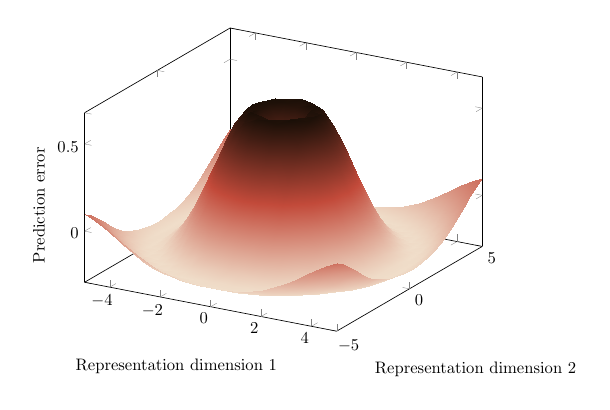
\begin{tikzpicture}[scale=0.6, thick]

    % Loss landscape illustration
    \begin{axis}[
        view={30}{30},
        xlabel={Representation dimension 1},
        ylabel={Representation dimension 2},
        zlabel={Prediction error},
        colormap={warm}{color=(wp-light) color=(wp-primary) color=(wp-dark)},
        width=10cm, height=8cm,
    ]
        \addplot3[
            surf,
            shader=interp,
            samples=25,
        ] {sin(deg(sqrt(x^2 + y^2)))/sqrt(x^2 + y^2 + 1)};
    \end{axis}

\end{tikzpicture}
\caption{Conceptual loss landscape of world model prediction error. Low-error regions
correspond to compact, accurate internal representations.}
\label{fig:landscape}
\end{figure}

\section{Conclusion}

World models represent a convergence of cognitive science, control theory, and deep learning,
offering a principled way to build agents that understand their environment through internal
simulation. The trajectory from Ha and Schmidhuber's three-component architecture to Hafner's
Dreamer family and transformer-based token prediction shows steady progress toward more capable,
general, and sample-efficient agents.

\begin{marginfigure}
\centering
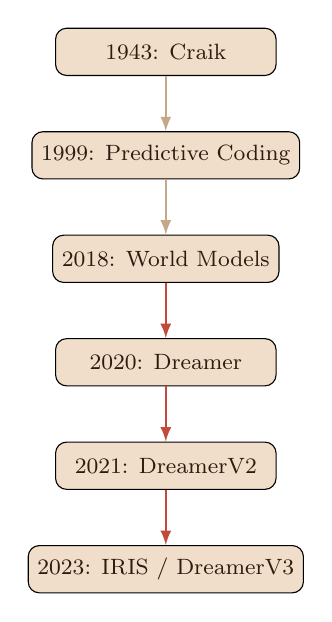
\begin{tikzpicture}[
    node distance=0.7cm, % Compact layout for narrow margin columns
    auto, 
    font=\footnotesize,
    >=latex
  ]
  
  % Global Style Definitions matching your design tokens
  \tikzset{
    era/.style={draw, fill=wp-light, rounded corners, minimum width=2.8cm, minimum height=0.6cm, text=wp-text, align=center}
  }

  % Chronological Vertical Node Structure
  \node (craik)   [era] {1943: Craik};
  \node (predict) [era, below=of craik] {1999: Predictive Coding};
  \node (wm)      [era, below=of predict] {2018: World Models};
  \node (dream)   [era, below=of wm] {2020: Dreamer};
  \node (dream2)  [era, below=of dream] {2021: DreamerV2};
  \node (iris)    [era, below=of dream2] {2023: IRIS / DreamerV3};

  % Chronological Connections with Latex Style Arrows
  \draw[->, wp-muted, thick] (craik) -- (predict);
  \draw[->, wp-muted, thick] (predict) -- (wm);
  \draw[->, wp-primary, thick] (wm) -- (dream);
  \draw[->, wp-primary, thick] (dream) -- (dream2);
  \draw[->, wp-primary, thick] (dream2) -- (iris);

\end{tikzpicture}
\caption{Timeline of world model development.}
\label{fig:timeline}
\end{marginfigure}

Key challenges remain in compositionality, long-horizon prediction, scalability, and causal
grounding. However, the convergence of ideas from neuroscience (predictive coding, free energy),
deep learning (VAEs, transformers), and control theory (model-based RL) suggests that world
models will play a central role in the next generation of intelligent systems.

\bibliographystyle{plainnat}
\bibliography{references}

\end{document}
